\documentclass{article}
\usepackage{graphicx} 
\usepackage[english,ukrainian]{babel}
\usepackage[letterpaper,top=2cm,bottom=2cm,left=3cm,right=3cm,marginparwidth=1.75cm]{geometry}
\usepackage{amsmath, graphicx, booktabs, listings, xcolor, tcolorbox, lipsum, siunitx, multirow, hyperref, pgfplots, inputenc}

\title{Застосування алгоритму дискретного логарифмування}
\date{}

\begin{document}

\maketitle

\section{Мета}
\quad Ознайомлення з алгоритмом дискретного логарифмування Сiльвера-Полiга-Геллмана. Практична реалiзацiя цього алгоритму. Пошук переваг,недолiкiв та особливостей застосування даного алгоритму дискретного логарифмування. Практична оцiнка складностi роботи алгоритму.

\section{Постановка задачі}
\quad Написати програму, що розв’язує задачу дисктерного логарифму шляхом звичайного перебору. Написати програму, що реалiзовує алгоритм Сiльвера-Полiга-Геллмана

\section{Приклад роботи програми}
\quad 
Testing SPH with a = 610053193922, b = 267528285417, p = 617047304681
digit length: 12, task type: 2, SPH result: x = 55966468673 (took 0.01 seconds)

\section{Замір часу роботи}
\quad 
\begin{figure}[htbp]
    \centering
    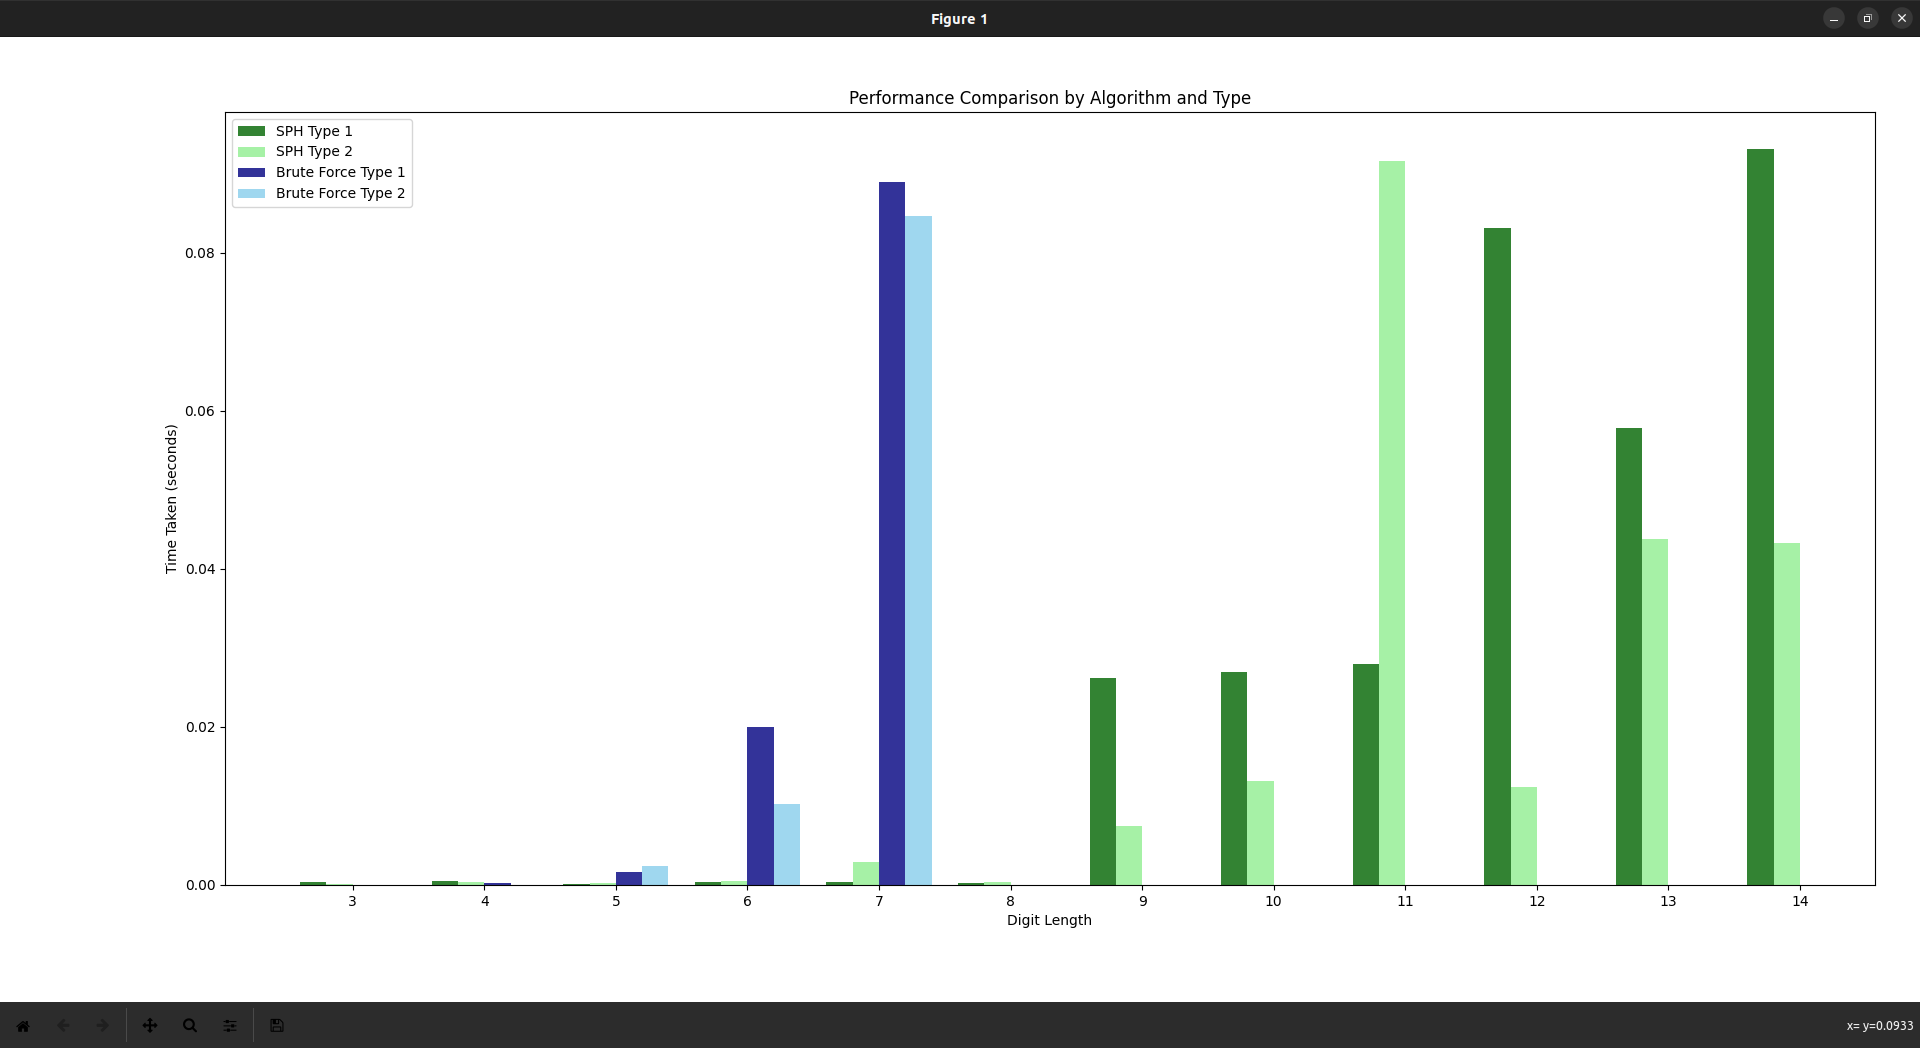
\includegraphics[width=1.0\textwidth]{time.png}
    \caption{час роботи}
    \label{fig:screenshot}
\end{figure}

\section{Висновок}
\quad
У цій роботі було розроблено програму для розв'язку задачі дискретного логарифму, автоматизовано заміри часу роботи розроблених алгоритмів, використовуючи надану програму, що генерує задачі різної довжини.
\end{document}
